\documentclass{article}
\usepackage{hyperref}
\usepackage{amsmath}
\usepackage{tikz}
\usetikzlibrary{patterns,decorations.pathreplacing} 
\usepackage[a4paper]{geometry}
\usepackage{fancyhdr}
\pagestyle{fancy}
\lhead{Das Fadenpendel}
\rhead{September 2025}
\begin{document}
\section{Fadenpendel}
\begin{minipage}[t]{\dimexpr\linewidth-4.5cm}
 \vspace*{0mm} 
 Ein \emph{Fadenpendel} besteht aus einem Gewicht, welches mit einem Faden über dem Boden befestigt wurde. Nach einmaliger Auslenkung schwingt hier der Winkel zwischen dem Faden und dem Faden der Ruhelage $\varphi$. 
 
Im Kräfteparallelogramm gilt
\[
 F_{r\ddot{u}ck} = F_G \cdot \sin{\varphi}
\]
Für kleine Winkel $\varphi$, wenn $l \gg \Delta y$, gilt in RAD ${\varphi = \sin{\varphi}}$. Wird dies eingesetzt und Umgeformt, so gilt
\[
 F_{r\ddot{u}ck} = m \cdot g \cdot y
\]
Weiterhin ist, der Definition eines Winkels in RAD nach, bei kleinen \par 
\end{minipage} 
\hfill
\begin{minipage}[t]{4.5cm}
 \vspace*{0mm} 
 \center 
 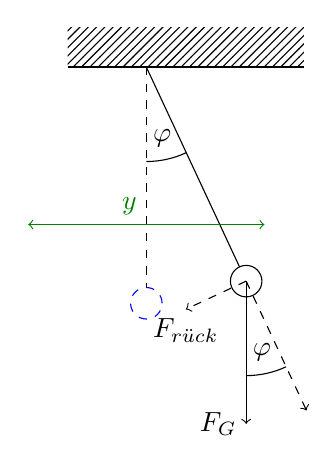
\begin{tikzpicture}
  \coordinate (mid) at (0,0); 
  \fill [pattern = north east lines] (-1,0) rectangle (2,0.5); 
  \draw (-1, 0) -- (2, 0); 
 
  \path (mid) ++({3*sin(155)}, {3*cos(155)}) coordinate (ball);
  \path (ball) ++({-0.2*sin(155)}, {-0.2*cos(155)}) coordinate (endline);
  \path (mid) ++(0, -3) coordinate (hypball);
  \path (hypball) ++(0, 0.2) coordinate (hypendline);
  \path (ball) ++({2*sin(245)*sin(90-65)}, {2*cos(245)*sin(90-65)}) coordinate (endfr);
  \path (ball) ++(0, {2*cos(155)}) coordinate (endfg);
  \path (ball) ++({2*sin(155)*sin(65)}, {2*cos(155)*sin(65)}) coordinate (endf);
 
  \draw (mid) -- (endline);
  % draw ball later to make it appear above the rest
  \draw[dashed] (mid) -- (hypendline);
  \draw[blue, dashed] (hypball) circle (0.2);
  \draw (0, -1.2) arc[start angle=-90, end angle=-65, radius=1.2];
  \draw (0.2, -0.9) node {$\varphi$}; 
  \draw[dashed, ->] (ball) -- (endfr) node[below] {$F_{r\ddot{u}ck}$};
  \draw[->] (ball) -- (endfg) node[left] {$F_{G}$};
 
  \draw[dashed, ->] (ball) -- (endf);
  \draw (ball) ++ (0, -1.2) arc[start angle=-90, end angle=-65, radius=1.2];
  \draw (ball) ++ (0.2, -0.9) node {$\varphi$};
 
  \draw (ball) circle (0.2);   
   
  \draw [<->, green!50!black] (-1.5, -2) -- (1.5, -2) node[midway, above left] {$y$};
 \end{tikzpicture} 
\end{minipage}
Winkeln $\varphi = \dfrac{y}{l}$. Es ist sich ein Kreis des Radius $l$ vorzustellen, wobei der Winkel $\varphi$ eine Kreisbogen $y$ umspannt. Es gilt letztendlich
\[
 F_{r\ddot{u}ck} = \frac{m \cdot g}{l} \cdot y
\] 
Weil die gefundene rücktreibende Kraft zur Auslenkung proportional ist, ist somit bewiesen, dass auch das Fadenpendel eine \hyperref[Mechanische Schwingungen]{harmonische Schwingung} darstellt.
 
Desweiteren kann die gefundene rücktreibende Kraft, wie bei der bestimmung der Schwingungsdauer eines \hyperref[Federoszilatoren]{Federoszilators} in
\[
 F_{r\ddot{u}ck} + m \cdot a = 0
\] 
eingesetzt werden, um eine Schwingungsdauer $T$ zu finden. Beim Fadenpendel folgt daraus
\[
 \boxed{
  T = 2\pi \cdot \sqrt{\frac{l}{g}}
 } 
\] 
 
\subsection{Energie}
An den Umkehrpunkten hat das Fadenpendel eine potenzielle Energie $E_{pot}$, während es sich durch die Ruhelage bewegt eine kinetische $E_{kin}$. Es gilt
\[
 E_{ges} = E_{pot} = E_{kin}
 \quad \text{mit} \quad 
 E_{pot} = m \cdot g \cdot h
 \quad \text{und} \quad
 \text{$h$ als Höhenunterschied} 
\] 
 
\end{document}